\documentclass[11pt]{article}
% Working draft. Will move to the ICML 2027 template once it is released.
% Every number is generated by src/collect_tables.py -> results/paper_numbers.json.
\usepackage[margin=1in]{geometry}
\usepackage[numbers,sort&compress]{natbib}
\usepackage{amsmath,amssymb,booktabs,graphicx,xcolor,multirow}
\usepackage[colorlinks=true,citecolor=blue,linkcolor=blue,urlcolor=blue]{hyperref}
\newcommand{\todo}[1]{\textcolor{red}{[TODO: #1]}}
\newcommand{\passk}[1]{\mathrm{pass@}#1}

\title{Pass@k Hides Differential Collapse:\\A Controlled Study of Post-Training in Medical Diagnosis}
\author{Jairam Hathwar\\University of Washington}
\date{Draft, \today}

\begin{document}
\maketitle

\begin{abstract}
A clinical diagnosis is a ranked differential, not a single answer, yet language models are mostly judged by whether their top answer is correct.
We study what post-training does to the rest of the differential.
We compare base models with their post-trained descendants under a controlled design: two base/instruct pairs (Qwen2.5-7B, Qwen3-8B), and three public medical models fine-tuned from the same parent with reinforcement learning, SFT with PPO, or distillation.
We evaluate them with 32 samples per case on DDXPlus, whose patients come with a reference differential, and on rare-disease cases from Phenopacket Store.
General post-training raises first-answer accuracy by 17 to 27 points but lowers coverage at larger sample budgets: base models are 10 to 15 points better at $\passk{32}$.
The post-trained models' sampled differentials collapse onto one or two diagnoses (answer entropy 0.18 vs.\ 1.31 for the base at $T{=}1$, against 1.87 for the reference), even though their top-1 calibration improves.
Medical RL applied after instruction tuning improves pass@$k$ at every $k$ but does not undo the collapse.
On rare disease, medical post-training raises stated confidence from 0.51 to 0.66--0.69 while accuracy stays below 2\%.
Single-answer metrics, including pass@$k$ at small $k$, therefore rate the post-trained models as strictly better while missing a large loss of diagnostic coverage.
\todo{training results sentence once E7 v2 completes}
\end{abstract}

%=====================================================================
\section{Introduction}
Clinicians reason over a differential diagnosis, a ranked set of conditions consistent with the presentation, and the conditions they keep in view determine which tests are ordered and which dangerous possibilities are ruled out.
Language-model evaluations in medicine nonetheless score a single answer: multiple-choice accuracy, top-1 diagnosis, or at most pass@$k$ for a small $k$.
Post-training, whether general instruction tuning and RLHF or domain-specific medical reinforcement learning and distillation, is reported to improve these scores~\citep{chen2024huatuogpto1,liu2025alphamed,huang2025m1}.
Work on reinforcement learning with verifiable rewards outside medicine suggests a cost: RL often sharpens a model's output distribution, so post-trained models win at $\passk{1}$ while their base models solve more problems given many samples~\citep{yue2025rlboundary,wu2025invisibleleash,oh2026sharpeningtax}.
Whether a similar trade-off holds for diagnosis, and whether it shows up in the differential rather than only in pass@$k$, has not been measured.

We measure it directly. Our design holds the pretrained model fixed and varies only the post-training:
(i) two base/instruct pairs, Qwen2.5-7B and Qwen3-8B, which isolate general post-training;
(ii) three public medical models fine-tuned from the same parent, Qwen2.5-7B-Instruct: AlphaMed (rule-based RL), HuatuoGPT-o1 (SFT then PPO), and m1 (SFT distillation).
We draw 32 samples per case and evaluate each model's sampled differentials against a reference distribution on DDXPlus~\citep{fansi2022ddxplus}, which ships a differential for every synthetic patient, and against an ontology on rare-disease cases from Phenopacket Store~\citep{danis2025phenopacketstore}.

\paragraph{Findings.}
\begin{enumerate}
\item \textbf{General post-training trades coverage for top-1 accuracy.} In both families the post-trained model is far better on its first answer (+17 to +27 points) but worse at larger sample budgets. Its pass@$k$ curve crosses the base model's at $k{\approx}4$--8, and at $k{=}32$ the base model leads by 10--15 points. All intervals exclude zero (\S\ref{sec:general}).
\item \textbf{The differential collapses, and single-answer metrics do not show it.} Post-trained models give 1.3--2.6 distinct top answers per 32 samples, against 3.8--8.3 for their base models. Their answer entropy is 0.11--0.49, against 0.78--1.59 for base models and 1.87 for the reference differential. This holds even when sampling at $T{=}1$. Their top-1 calibration is \emph{better}, so on every single-answer metric they look strictly superior (\S\ref{sec:collapse}).
\item \textbf{Medical RL on an instruction-tuned model adds accuracy without undoing the collapse.} AlphaMed improves on its parent at every $k$ (+3.9 at $k{=}1$, +8.4 at $k{=}32$), so we see no sharpening tax at the medical stage. Its answer diversity matches its parent's, which is already collapsed (\S\ref{sec:medical}).
\item \textbf{On rare disease, medical post-training increases overconfidence.} With accuracy below 2\% for every model, mean stated confidence rises from 0.51 for the parent to 0.66--0.69 for its RL-trained descendants (\S\ref{sec:rare}).
\end{enumerate}
\todo{fourth contribution: GRPO with distribution-level rewards vs.\ set-based rewards~\citep{puri2026beyondmode}, once E7 v2 is stable}

%=====================================================================
\section{Related work}
\paragraph{What RL does to a model's output distribution.}
\citet{yue2025rlboundary} find that RL with verifiable rewards improves $\passk{1}$ on math and code while base models win at large $k$.
\citet{wu2025invisibleleash} argue that RLVR mostly reweights solutions already in the base model's support.
\citet{oh2026sharpeningtax} document a ``sharpening tax'' across 14 base/post-trained pairs on agentic benchmarks.
In contrast, \citet{cheng2025guru} report that RL expands the boundary on domains under-represented in pretraining.
In medicine, the only pass@$k$ analysis we know of studies vision-language models and finds that RL mainly sharpens~\citep{jeddi2026medvlmrl}.
We give the first text-only medical analysis, and we measure the differential directly rather than only pass@$k$.

\paragraph{Diversity loss from alignment.}
Instruction tuning and RLHF reduce output diversity~\citep{kirk2024rlhfdiversity,west2025basemodels}. Related work explains this as typicality bias~\citep{zhang2025verbalized} and documents cross-model homogeneity~\citep{jiang2025hivemind}.
We quantify this loss against a clinical reference distribution.

\paragraph{Medical reasoning models and calibration.}
Medical post-training recipes include verifier-guided SFT and PPO~\citep{chen2024huatuogpto1}, minimalist rule-based RL~\citep{liu2025alphamed}, and test-time-scaling distillation~\citep{huang2025m1}.
Reward models and RL tend to favor confident answers~\citep{leng2025taming,damani2025rlcr}, and reasoning models are often overconfident~\citep{mei2025reasoninguncertainty}.
We show that this overconfidence appears in public medical descendants of one parent, on rare disease.

\paragraph{Differential diagnosis benchmarks and distributional RL.}
DDXPlus~\citep{fansi2022ddxplus} was introduced for automatic diagnosis systems trained on differentials~\citep{fansi2022casande}. Recent LLM evaluations on it score hierarchical top-$k$ accuracy~\citep{h-ddx2025}.
\citet{puri2026beyondmode} train models with GRPO to output several answers per forward pass, rewarding coverage of a gold \emph{set} and set-level calibration, and evaluate on DDXPlus.
We instead measure collapse against the reference \emph{distribution} across public post-trained model families.
\todo{position our training study relative to Puri et al.}

%=====================================================================
\section{Experimental setup}\label{sec:setup}
\paragraph{Tasks.}
\textbf{DDXPlus}~\citep{fansi2022ddxplus}: synthetic patients produced by a rule-based medical knowledge base. Each patient has a true pathology and a reference differential, a probability distribution over the 49 conditions.
We use 980 test patients, 20 per condition. Each patient's coded symptoms and history are rendered as a short vignette; we fix known mistranslations in the English evidence descriptions.
The prompt lists all 49 conditions and asks for the five most likely, with probabilities, as JSON.
\textbf{Phenopacket Store}~\citep{danis2025phenopacketstore} (v0.1.27): published rare-disease cases annotated with HPO phenotypes and an OMIM diagnosis.
We use a disease-balanced set of 500 cases covering 418 diseases. Each case is a vignette of present and absent phenotypes, and the model is asked for an open-ended differential.
Answers are graded by mapping names to Mondo; we credit an exact match, and separately a ``related'' match to a specific ancestor group or subtype.

\paragraph{Models.} Table~\ref{tab:models}. All checkpoints are public. For the medical models we verified the parent model from each released configuration.

\begin{table}[t]
\centering\small
\begin{tabular}{llll}
\toprule
Model & Parent & Post-training & Role \\
\midrule
Qwen2.5-7B & n/a & none (pretrained) & base \\
Qwen2.5-7B-Instruct & Qwen2.5-7B & general SFT + RLHF & instruct; medical parent \\
AlphaMed-7B~\citep{liu2025alphamed} & Qwen2.5-7B-Instruct & rule-based RL & medical \\
HuatuoGPT-o1-7B~\citep{chen2024huatuogpto1} & Qwen2.5-7B-Instruct & SFT + PPO (verifier) & medical \\
m1-7B-23K~\citep{huang2025m1} & Qwen2.5-7B-Instruct & SFT distillation & medical \\
Qwen3-8B-Base & n/a & none (pretrained) & base \\
Qwen3-8B & Qwen3-8B-Base & general post-training & instruct \\
\bottomrule
\end{tabular}
\caption{Models studied. Each pair or family shares its pretrained weights, so differences reflect post-training.}
\label{tab:models}
\end{table}

\paragraph{Sampling.}
We draw $n{=}32$ samples per case with vLLM, at $T{=}0.7$, top-$p$ 0.95, and at $T{=}1.0$, top-$p$ 1.0 (sampling from the model's own distribution). All models use their chat template and the same prompt.
Completions are capped at 4,096 tokens (8,192 for m1, whose long reasoning otherwise truncates), and generation stops at the end-of-turn token.
We take the last valid JSON list in each completion. Unparsable completions count as incorrect; this affects mainly base models (11--19\%), so base-model pass@$k$ is a lower bound.

\paragraph{Metrics.}
\emph{pass@$k$}: the unbiased estimator of \citet{chen2021codex} on the top-1 answer of each sample.
\emph{Distinct} and \emph{entropy}: the number of distinct top-1 diagnoses across a case's 32 samples, and the entropy of their empirical distribution, averaged over cases.
On DDXPlus, \emph{TV}: total-variation distance between this empirical distribution and the reference differential.
\emph{Coverage@$k$}: the expected share of the reference differential's probability mass covered by the distinct top-1 answers in $k$ random samples.
\emph{Calibration}: expected calibration error (10 bins) of the stated top-1 probability against top-1 correctness.
Differences come with 95\% paired-bootstrap intervals over cases (2,000 resamples).

%=====================================================================
\section{Results}

\subsection{General post-training trades coverage for top-1 accuracy}\label{sec:general}
Table~\ref{tab:pairs} and Figure~\ref{fig:passk} compare each base model with its post-trained counterpart on DDXPlus.
In both families the post-trained model is much better on its first answer: +27.5 points for Qwen3 and +22.2 for Qwen2.5 at $T{=}1$ (intervals $[+25.3,+29.6]$ and $[+20.1,+24.4]$).
The advantage shrinks with $k$ and reverses: the curves cross at $k{\approx}4$--8, and at $k{=}32$ the base model leads by 14.6 points (Qwen3, $[+12.2,+17.1]$) and 10.0 points (Qwen2.5, $[+7.1,+12.8]$).
The pattern is the same at $T{=}0.7$ for Qwen3, crossing at $k{=}4$ with a base lead of 12.2 points at $k{=}32$ ($[+9.9,+14.9]$).
Unparsable base-model samples count as wrong, so these gaps are lower bounds.
\todo{Qwen2.5 base pair on all 980 cases (currently 811); Qwen2.5 base at $T{=}0.7$.}

\begin{table}[t]
\centering\small
\setlength{\tabcolsep}{4pt}
\begin{tabular}{llcccccccc}
\toprule
Pair & Model & $\passk{1}$ & $\passk{32}$ & Distinct & Entropy & TV$\downarrow$ & Cov@32 & ECE$\downarrow$ \\
\midrule
\multirow{2}{*}{Qwen3-8B, $T{=}1$} & base & 0.282 & \textbf{0.789} & \textbf{6.60} & \textbf{1.31} & \textbf{0.712} & \textbf{0.407} & 0.214 \\
 & post-trained & \textbf{0.556} & 0.643 & 1.53 & 0.18 & 0.783 & 0.236 & \textbf{0.061} \\
\midrule
\multirow{2}{*}{Qwen2.5-7B, $T{=}1$} & base & 0.235 & \textbf{0.757} & \textbf{8.32} & \textbf{1.59} & \textbf{0.712} & \textbf{0.426} & 0.309 \\
 & instruct & \textbf{0.457} & 0.657 & 2.63 & 0.49 & 0.761 & 0.290 & \textbf{0.137} \\
\midrule
\multirow{2}{*}{Qwen3-8B, $T{=}0.7$} & base & 0.388 & \textbf{0.730} & \textbf{3.76} & \textbf{0.78} & \textbf{0.750} & \textbf{0.322} & 0.121 \\
 & post-trained & \textbf{0.558} & 0.607 & 1.27 & 0.11 & 0.793 & 0.217 & \textbf{0.063} \\
\bottomrule
\end{tabular}
\caption{DDXPlus, 32 samples per case (980 cases; 811 for Qwen2.5 at $T{=}1$, \todo{complete}). The reference differential has mean entropy 1.87. Distinct and entropy refer to the top-1 answers across samples; Cov@32 is the share of reference probability mass covered by those answers. ECE is for the stated top-1 probability.}
\label{tab:pairs}
\end{table}

\begin{figure}[t]
\centering
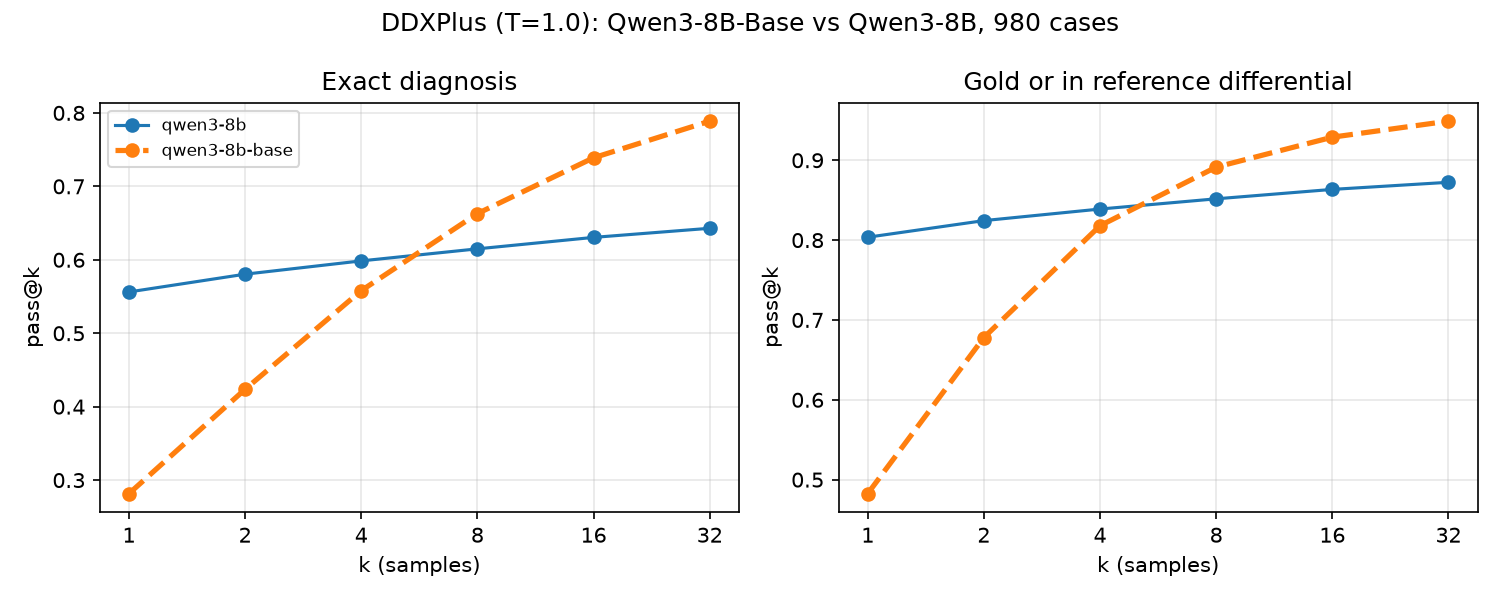
\includegraphics[width=0.49\linewidth]{figures/passk_qwen3_t1.png}\hfill
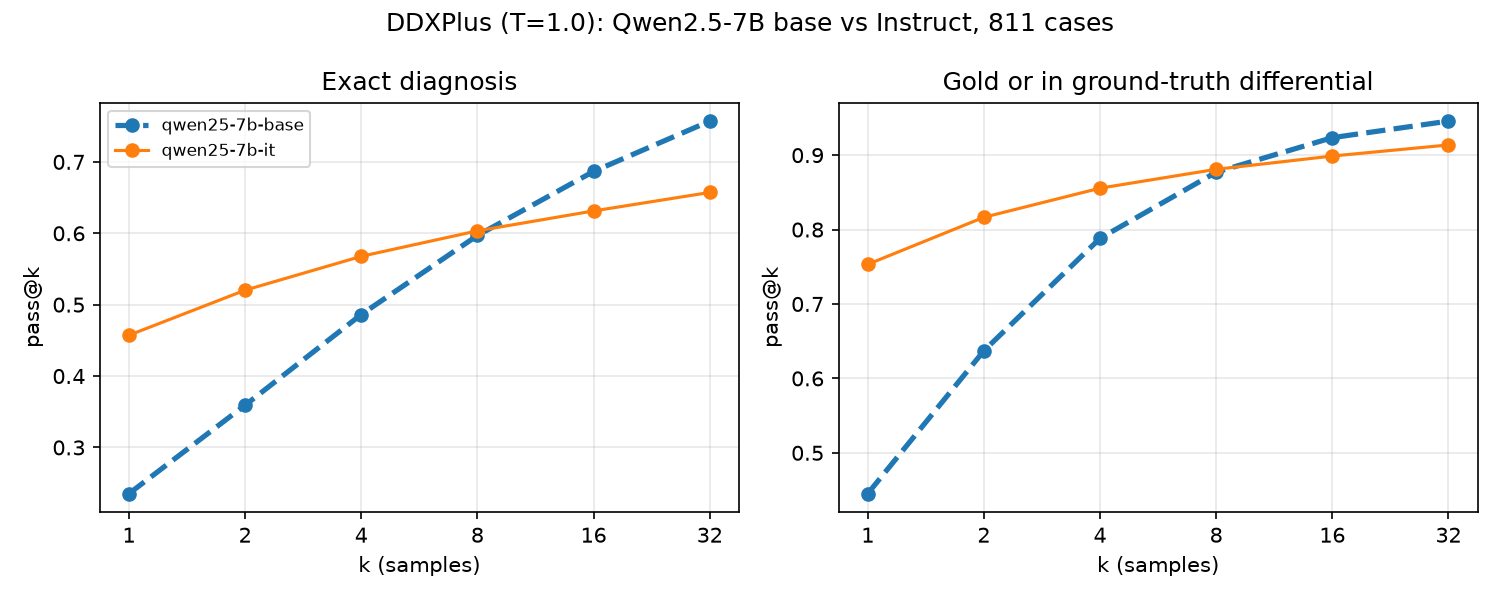
\includegraphics[width=0.49\linewidth]{figures/passk_qwen25_t1.png}
\caption{pass@$k$ on DDXPlus at $T{=}1$. Left: Qwen3-8B-Base vs.\ Qwen3-8B. Right: Qwen2.5-7B base vs.\ Instruct. In each, the post-trained model wins at small $k$ and loses at large $k$. Right panels of each plot count a sample as correct if its answer is the gold condition or appears in the reference differential. \todo{redraw as one paper-style figure with CIs}}
\label{fig:passk}
\end{figure}

\subsection{The differential collapses, while top-1 calibration improves}\label{sec:collapse}
The gap at large $k$ reflects a collapsed differential.
Across 32 samples, post-trained models name 1.3--2.6 distinct diagnoses per case, against 3.8--8.3 for their base models.
Their answer entropy is 0.11--0.49, against 0.78--1.59 for base models and 1.87 for the reference differential (Table~\ref{tab:pairs}).
Sampling at $T{=}1$ widens the base models' answers but barely changes the post-trained models' (Qwen3 entropy 0.11 at $T{=}0.7$, 0.18 at $T{=}1$), so the collapse lives in the model's own distribution rather than in the decoding settings.
As a result, post-trained models cover less of the reference differential: 0.24 vs.\ 0.41 of its probability mass at $k{=}32$ for Qwen3, and 0.29 vs.\ 0.43 for Qwen2.5.
Their top-1 calibration, however, is markedly better (ECE 0.06 vs.\ 0.21 and 0.14 vs.\ 0.31).
On every single-answer criterion (accuracy, small-$k$ pass@$k$, calibration), the post-trained model therefore looks strictly better, and the loss of diagnostic breadth is invisible.
\paragraph{Which diagnoses drop out?}
For each case and each condition that the reference differential weights at least 0.1, we ask whether the model names that condition as its top answer in at least one of its 32 samples. We call this \emph{considering} the condition.
We group the 49 conditions by DDXPlus severity (1 = most severe).
Post-training lowers consideration in every tier (Table~\ref{tab:severity}), and the severe ``can't-miss'' tier is not spared.
For the 17 severity-1--2 conditions (e.g.\ NSTEMI/STEMI, acute pulmonary edema, anaphylaxis, pulmonary embolism, unstable angina), consideration falls from 0.45 to 0.27 for Qwen3 and from 0.52 to 0.34 for Qwen2.5 at $T{=}1$. The differences are $-18.4$ $[-20.8,-15.9]$ and $-18.2$ $[-21.4,-15.2]$ points.
Some diagnoses disappear from the top answer almost entirely.
Qwen2.5-7B-Instruct names unstable angina as its top answer in one of 107 eligible cases, where its base model does in 47\%. When unstable angina is the true pathology, $\passk{32}$ falls from 1.00 to 0.00. Stable angina (0.89 to 0.06) and myocarditis (0.41 to 0.00) follow the same pattern.
These conditions are not forgotten: they still appear lower in the listed differential (unstable angina in 50\% of eligible cases, against 95\% for the base model). The model ranks them but no longer commits to them.
At the same time, post-trained models concentrate on a few salient ``attractor'' diagnoses.
Qwen2.5-7B-Instruct gives NSTEMI/STEMI as its top answer in 13.1\% of samples, against a reference rate of 4.4\% and 6.4\% for its base model. It also over-predicts pulmonary embolism (8.2\% vs.\ 3.2\%) and pneumonia (8.0\% vs.\ 2.4\%).
Chest-pain presentations thus collapse onto the most dangerous candidate. That raises its accuracy (NSTEMI $\passk{1}$ 0.99 vs.\ 0.44) at the cost of the alternatives, which is a defensible triage bias but not a differential.

\begin{table}[t]
\centering\small
\begin{tabular}{lcccc}
\toprule
 & \multicolumn{3}{c}{Considered@32 (base $\rightarrow$ post-trained)} & \\
Comparison & Severe (1--2) & Moderate (3) & Mild (4--5) & \\
\midrule
Qwen3-8B, $T{=}1$ & 0.45 $\rightarrow$ 0.27 & 0.50 $\rightarrow$ 0.32 & 0.45 $\rightarrow$ 0.20 & \\
 & \footnotesize{$-18.4$ [$-20.8,-15.9$]} & \footnotesize{$-18.1$ [$-20.7,-15.7$]} & \footnotesize{$-24.2$ [$-27.0,-21.4$]} & \\
Qwen2.5-7B, $T{=}1$ & 0.52 $\rightarrow$ 0.34 & 0.50 $\rightarrow$ 0.38 & 0.39 $\rightarrow$ 0.23 & \\
 & \footnotesize{$-18.2$ [$-21.4,-15.2$]} & \footnotesize{$-12.3$ [$-15.2,-9.4$]} & \footnotesize{$-15.4$ [$-18.2,-12.5$]} & \\
Qwen3-8B, $T{=}0.7$ & 0.34 $\rightarrow$ 0.24 & 0.44 $\rightarrow$ 0.29 & 0.31 $\rightarrow$ 0.18 & \\
 & \footnotesize{$-9.8$ [$-11.8,-7.9$]} & \footnotesize{$-15.8$ [$-18.2,-13.5$]} & \footnotesize{$-13.4$ [$-15.8,-11.1$]} & \\
\midrule
Instruct $\rightarrow$ AlphaMed, $T{=}0.7$ & 0.28 $\rightarrow$ 0.32 & 0.32 $\rightarrow$ 0.34 & 0.17 $\rightarrow$ 0.21 & \\
 & \footnotesize{$+4.3$ [$+2.0,+6.6$]} & \footnotesize{$+2.2$ [$+0.3,+4.1$]} & \footnotesize{$+3.9$ [$+2.4,+5.5$]} & \\
\bottomrule
\end{tabular}
\caption{Share of (case, condition) pairs with reference probability $\geq 0.1$ in which the condition is a top-1 answer in at least one of 32 samples, by DDXPlus severity. Second rows give differences in points with 95\% case-bootstrap intervals. Post-training lowers consideration in every tier, including the can't-miss tier; medical RL slightly raises it. (Qwen2.5 at $T{=}1$: 811 cases, \todo{complete}.)}
\label{tab:severity}
\end{table}

\begin{figure}[t]
\centering
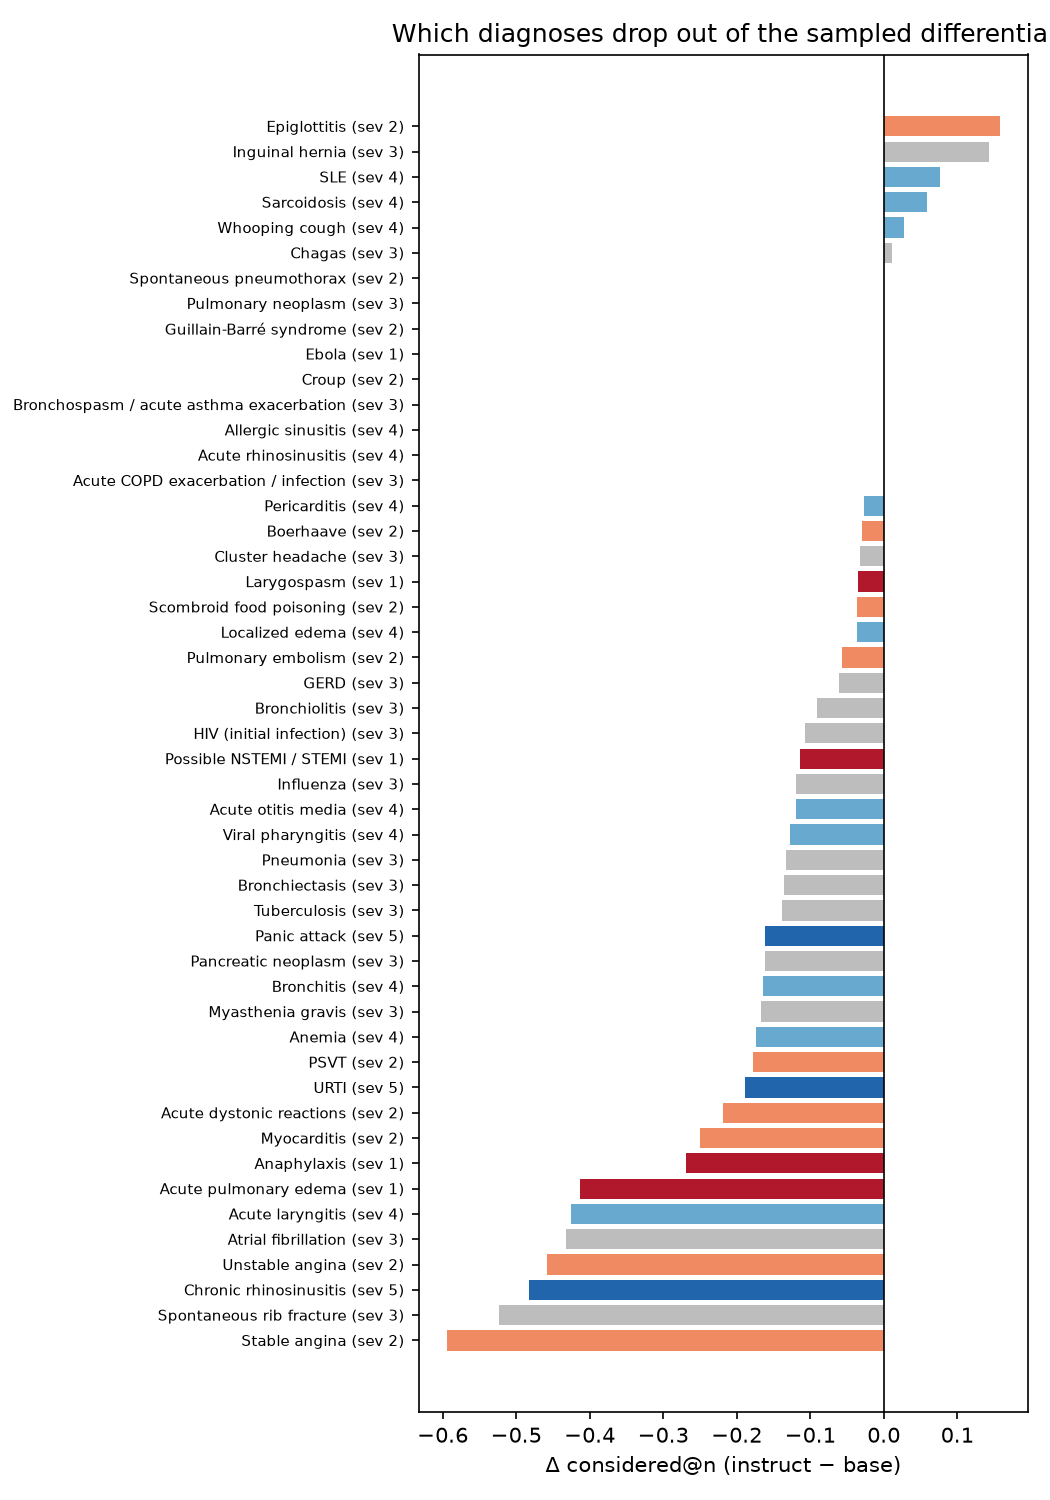
\includegraphics[width=0.62\linewidth]{figures/per_condition_qwen25_t1.png}
\caption{Change in consideration per condition, Qwen2.5-7B-Instruct minus its base model ($T{=}1$), colored by severity (red = most severe). Angina, acute pulmonary edema, anaphylaxis and myocarditis are among the largest drops. \todo{paper-style redraw}}
\label{fig:percond}
\end{figure}

\subsection{Medical post-training on an instruction-tuned model}\label{sec:medical}
Applied after instruction tuning, medical RL does not cost coverage. AlphaMed improves on its parent at every $k$ (Figure~\ref{fig:alphamed}): +3.9 points at $k{=}1$ ($[+2.2,+5.5]$), widening to +8.4 at $k{=}32$ ($[+6.0,+10.6]$). It reaches at least one correct sample for 47 of 49 conditions, against 39 for its parent.
It does not restore breadth, though: distinct answers (1.87 vs.\ 1.82), entropy (0.29 vs.\ 0.30), and coverage (0.27 vs.\ 0.24) stay at the instruction-tuned level, far below the base model.
AlphaMed also names off-list conditions more often than its parent, a mild loss of instruction following.
By condition, AlphaMed slightly \emph{raises} consideration in every severity tier (+2.2 to +4.3 points; Table~\ref{tab:severity}). It still loses acute pulmonary edema (0.31 to 0.13), and it introduces an attractor of its own: spontaneous pneumothorax as the top answer in 10.3\% of samples, against 4.3\% for its parent and a reference rate of 1.0\%.
Medical post-training thus operates on an already collapsed distribution. The collapse comes from the general post-training stage.
\todo{HuatuoGPT-o1 (SFT+PPO) and m1 (SFT distillation) on DDXPlus; on Phenopackets HuatuoGPT is narrower and m1 broader than the parent.}

\begin{figure}[t]
\centering
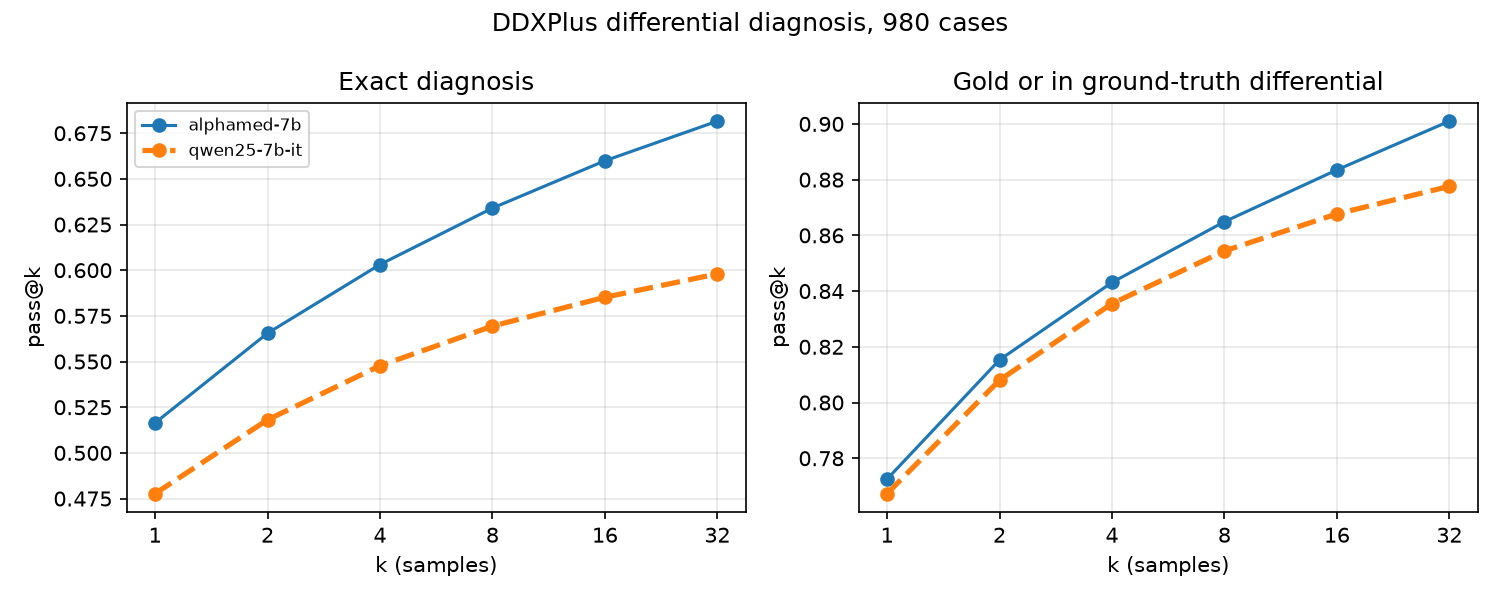
\includegraphics[width=0.6\linewidth]{figures/passk_alphamed_t07.png}
\caption{DDXPlus at $T{=}0.7$: Qwen2.5-7B-Instruct (dashed) vs.\ its RL-trained medical descendant AlphaMed. The gap widens with $k$, so there is no sharpening tax at the medical stage.}
\label{fig:alphamed}
\end{figure}

\subsection{Rare disease: overconfidence without accuracy}\label{sec:rare}
On 500 Phenopacket Store cases covering 418 diseases, every 7B model is near the floor: $\passk{1}$ is 1.3--1.9\% and $\passk{32}$ is 6--7\%, and differences in pass@$k$ are within noise.
Stated confidence is not near the floor. The parent model states a mean top-1 probability of 0.51, and its medical descendants state 0.66 (HuatuoGPT-o1) and 0.69 (AlphaMed), while their accuracy stays at 1.9\%. ECE accordingly rises from 0.50 to 0.64--0.67.
Medical post-training thus increases overconfidence exactly where the model is out of its depth.
HuatuoGPT-o1 is also the narrowest model here (9.4 distinct answers per 32 samples, against 11.5 for its parent).
Cases from older publications are much easier than recent ones, which suggests memorization; we report results by publication era \todo{era table: $\le$2022 vs.\ 2023--24 vs.\ 2025+; m1 with an 8k token budget; full 1,401-case set}.

%=====================================================================
\section{Limitations}
DDXPlus is synthetic: its reference differential is the posterior of a rule-based engine, and the true pathology is ranked first for only about 70\% of patients \todo{verify this figure in \citet{fansi2022ddxplus}}, so we treat TV and coverage as distance to a \emph{reference} posterior rather than to clinical truth.
Base models fail to produce parsable answers more often. We count these as errors, which biases against base models and makes our gaps conservative.
All models so far are Qwen-family 7--8B models evaluated with a single prompt format. \todo{Llama-3.1-8B family; prompt variants.}
Phenopacket cases are drawn from published literature and may be in pretraining data, which we partly address with era splits.
We do not evaluate clinical utility with clinicians.

\bibliographystyle{plainnat}
\bibliography{refs}
\end{document}
